%%%%%%%%%%%%%%%%%%%%%%%%%%%%%%%%%%%%%%%%%%%%%%%%%%%%%%%%%%%%%%%%%%%%%%
% How to use writeLaTeX: 
%
% You edit the source code here on the left, and the preview on the
% right shows you the result within a few seconds.
%
% Bookmark this page and share the URL with your co-authors. They can
% edit at the same time!
%
% You can upload figures, bibliographies, custom classes and
% styles using the files menu.
%
%%%%%%%%%%%%%%%%%%%%%%%%%%%%%%%%%%%%%%%%%%%%%%%%%%%%%%%%%%%%%%%%%%%%%%



\documentclass[12pt]{article}

\usepackage{sbc-template} 
\usepackage{graphicx,url}

%\usepackage[brazil]{babel}   
\usepackage[utf8]{inputenc}  

     
\sloppy

\title{Vpns e seus usos na computação moderna\\ Documentos e Resumo}

\author{Pedro Henrique Bufulin de Almeida \inst{1}, Gabriel Solis Corrêa\inst{2},\\ TODO - Adicionar Nomes - Flávio Rech
  Wagner\inst{1}, Jomi F. Hübner\inst{3} }


\address{Faculdade de Computação -- Universidade Federal de Uberlândia
  (UFU)\\
  Caixa Postal 593 -- CEP 38.400-902 -- Uberlândia -- MG -- Brazil
  \email{gsolis.comp@gmail.com, TODO - Adicionem o email de vcs}
}

\begin{document} 

\maketitle
     
\begin{resumo} 
  Presente Artigo visa explorar as VPNs, seus usos na computação moderna
  e ferramentas relacionadas, além de conceituar o termo VPN. Serão realizados
  e documentados testes utilizando a ferramenta OpenVPN em um sistema de máquinas Ubuntu,
  hospedados nos servidores da Digital Ocean, para observar o funcionamento e as
  limitações de uma VPN.
\end{resumo}

\section{Introdução}

% All full papers and posters (short papers) submitted to some SBC conference,
% including any supporting documents, should be written in English or in
% Portuguese. The format paper should be A4 with single column, 3.5 cm for upper
% margin, 2.5 cm for bottom margin and 3.0 cm for lateral margins, without
% headers or footers. The main font must be Times, 12 point nominal size, with 6
% points of space before each paragraph. Page numbers must be suppressed.

% Full papers must respect the page limits defined by the conference.
% Conferences that publish just abstracts ask for \textbf{one}-page texts.

\section{Desenvolvimento}

\subsection{Configurado uma VPN utilizando OpenVPN}

Para que seja possível implementar uma VPN como neste exemplo, você precisará
de uma máquina rodando Ubuntu versão 18.04. Por questões de praticidade, não será
visto com profundidade todo o processo de instalação das ferramentas que serão usadas, sendo algumas 
apenas mencionadas cabendo ao leitor descobrir como instalá-las. Além do servidor mencionado,
o ideal seria ter uma outra máquina para ser a autoridade de certificação (CA), para evitar
que um agressor capaz de se infiltrar no servidor consiga acessar a chave privada
e assinar novos certificados. 

\subsection{Instalando os programas necessários}

O primeiro passo é instalar o \emph{OpenVPN} que está disponível nos repositórios padrão do ubuntu.
Em seguida, instale \emph{EasyRCA} tanto na máquina CA quanto no servidor que servira o VPN.
O repositório deste programa encontra-se no github no mesmo repositório do \emph{OpenVPN}. 
A versão a ser utilizada é a 3.0.8.

\subsection{Configurando as variáveis e construindo o CA}

No máquina que contém o CA, entre no diretório onde foi extraído o \emph{EasyRCA}. copie o conteúdo
do arquivo \texttt{vars.example} para um outro arquivo onde serão armazenadas as variáveis. Atualize
os valores de acordo com suas informações, feche e salve o arquivo. 

Dentro do da mesma pasta, existe um\emph{script} chamado \texttt{easyrca}. Execute-o da seguinte
maneira: \texttt{./easyrsa init-pki}. Isso irá iniciar a infraestrutura de chaves públicas no servidor CA.
Se der tudo certo, deve surgir um diretório chamado \texttt{pki}. Em seguida, chame o script anterior 
novamente mas dessa vez com a opção \texttt{build-ca}. Isso irá construir a CA e criar
dois arquivos importantes. Um deles é um certificado público que no contexto de uma VPN para informar
ao servidor e ao cliente que ambos fazem parte da mesma rede. Isso serve como defesa de ataques 
do tipo \emph{man-in-the-middle} 



\section{Discussão}

% Section titles must be in boldface, 13pt, flush left. There should be an extra
% 12 pt of space before each title. Section numbering is optional. The first
% paragraph of each section should not be indented, while the first lines of
% subsequent paragraphs should be indented by 1.27 cm.

\section{Considerações Finais}


% Figure and table captions should be centered if less than one line
% (Figure~\ref{fig:exampleFig1}), otherwise justified and indented by 0.8cm on
% both margins, as shown in Figure~\ref{fig:exampleFig2}. The caption font must
% be Helvetica, 10 point, boldface, with 6 points of space before and after each
% caption.

% \begin{figure}[ht]
% \centering
% 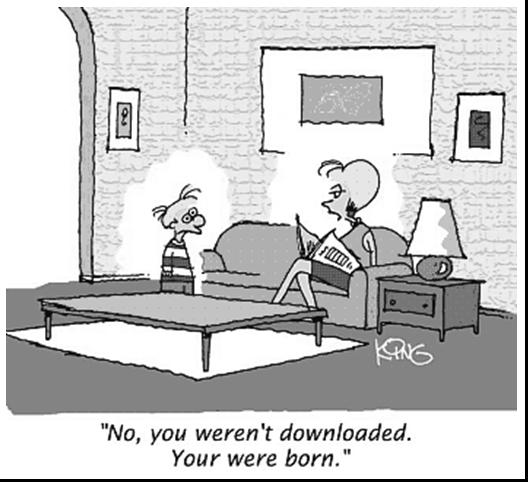
\includegraphics[width=.5\textwidth]{fig1.jpg}
% \caption{A typical figure}
% \label{fig:exampleFig1}
% \end{figure}

% \begin{figure}[ht]
% \centering
% 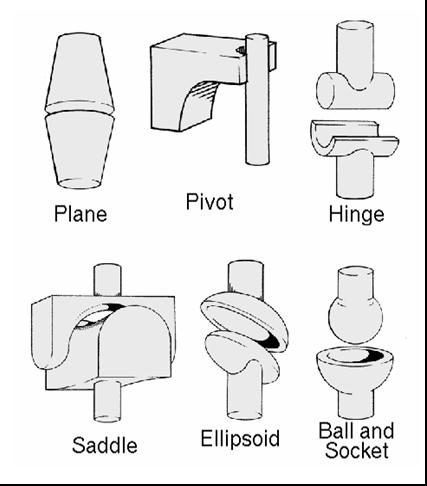
\includegraphics[width=.3\textwidth]{fig2.jpg}
% \caption{This figure is an example of a figure caption taking more than one
%   line and justified considering margins mentioned in Section~\ref{sec:figs}.}
% \label{fig:exampleFig2}
% \end{figure}

% In tables, try to avoid the use of colored or shaded backgrounds, and avoid
% thick, doubled, or unnecessary framing lines. When reporting empirical data,
% do not use more decimal digits than warranted by their precision and
% reproducibility. Table caption must be placed before the table (see Table 1)
% and the font used must also be Helvetica, 10 point, boldface, with 6 points of
% space before and after each caption.

% \begin{table}[ht]
% \centering
% \caption{Variables to be considered on the evaluation of interaction
%   techniques}
% \label{tab:exTable1}
% 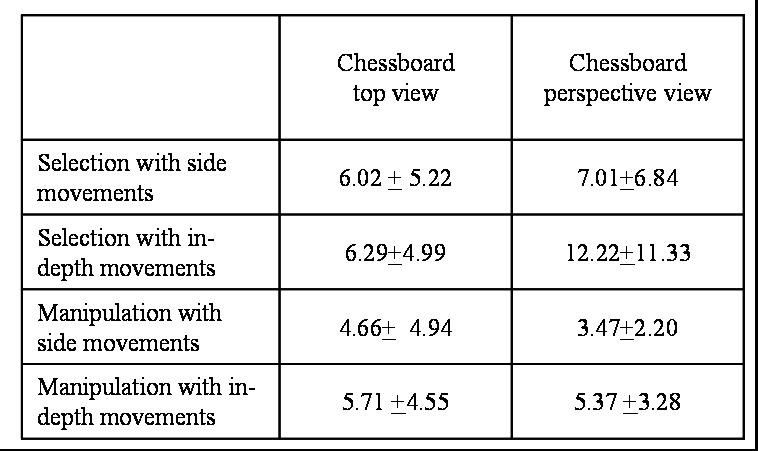
\includegraphics[width=.7\textwidth]{table.jpg}
% \end{table}

\section{Referências}

Bibliographic references must be unambiguous and uniform.  We recommend giving
the author names references in brackets, e.g. \cite{knuth:84},
\cite{boulic:91}, and \cite{smith:99}.

The references must be listed using 12 point font size, with 6 points of space
before each reference. The first line of each reference should not be
indented, while the subsequent should be indented by 0.5 cm.

\bibliographystyle{sbc}
\bibliography{sbc-template}

\end{document}
